\definecolor{c1}{HTML}{0072B2}
\definecolor{c2}{HTML}{009E73}
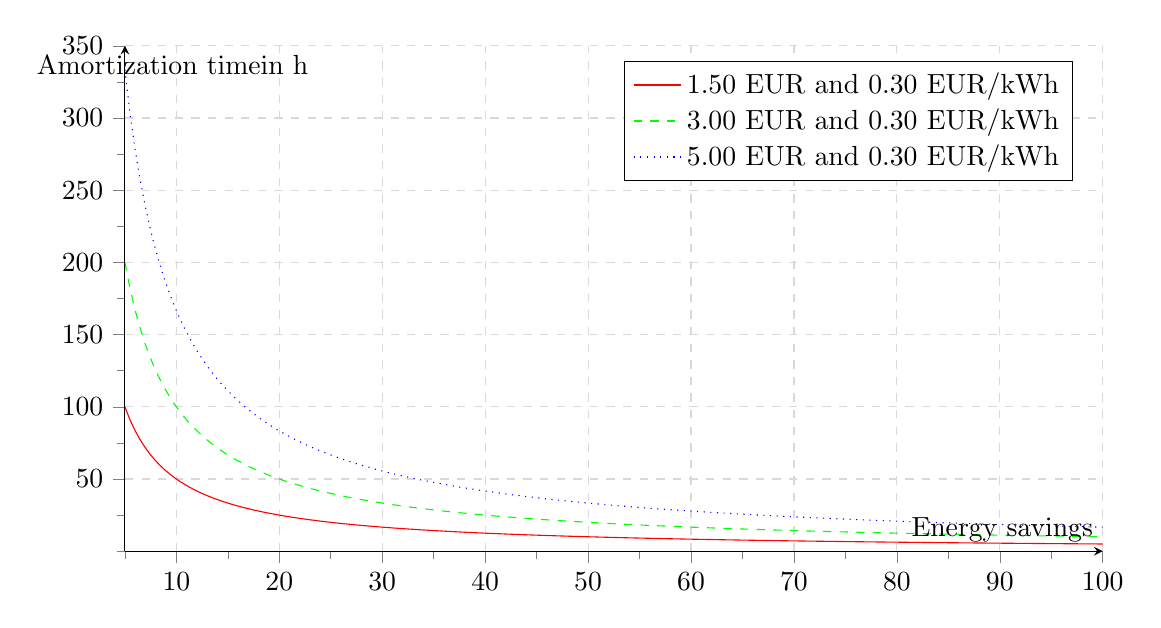
\begin{tikzpicture}
    \tikzstyle{training}=[c1, thick,samples=200,dashed]
    \tikzstyle{testing}=[c2, thick,samples=200]
    \begin{axis}[
        legend pos=north east,
        legend cell align=left,
        axis x line=middle,
        axis y line=middle,
        grid = major,
        width=14cm,
        height=8cm,
        grid style={dashed, gray!30},
        xmin=5,       % start the diagram at this x-coordinate
        xmax=100,    % end   the diagram at this x-coordinate
        ymin=0,       % start the diagram at this y-coordinate
        ymax=350,   % end   the diagram at this y-coordinate
        axis background/.style={fill=white},
        xlabel=Energy savings,
        ylabel={Amortization time\\in h},
        y label style={at={(-0.1,1.0)}},
        tick align=outside,
        minor tick num=-3,
        tension=0.08]

        \addplot[domain=5:100, red, solid, samples=200] {1.50 / (0.003 * x)};
        \addplot[domain=5:100, green, dashed, samples=200] {3.00 / (0.003 * x)};
        \addplot[domain=5:100, blue, dotted, samples=200] {5.00 / (0.003 * x)};

      %\draw[dashed, very thick] (axis cs:50,0.0) -- (axis cs:50,0.3);
      %\draw[decoration={text along path, text={overfitting}, text align={center}}, decorate] (axis cs:51,0.16) -- (axis cs:90,0.16);
      %\draw[-{latex[scale=3.0]}, very thick] (axis cs:51,0.15) -- (axis cs:90,0.15);

      \addlegendentry{1.50 EUR and 0.30 EUR/kWh}
      \addlegendentry{3.00 EUR and 0.30 EUR/kWh}
      \addlegendentry{5.00 EUR and 0.30 EUR/kWh}
    \end{axis}
\end{tikzpicture}
